\documentclass[12pt,a4paper]{article}
\usepackage[utf8]{inputenc}
\usepackage[T1]{fontenc}
\usepackage{amsmath}
\usepackage{amsfonts}
\usepackage{amssymb}
\usepackage{graphicx}
\usepackage{physics}
\usepackage{cite}
\usepackage{caption}
\usepackage{subcaption}
\usepackage{hyperref}
\usepackage{comment}
\linespread{1.2}
\usepackage[a4paper,top=3cm,bottom=3cm,left=3cm,right=3cm]{geometry}

\title{On the ground state degeneracy of the Quantum Ising Model}
\author{}
\begin{document}
	\maketitle

We want to characterize the ground state of the 1D Quantum Ising Model, we will focus in particular on his entanglement content, his symmetry properties, on the differences beetween the Classical and Quantum symmetry breaking and some numerical issues.

\section{Some definitions}
The \textbf{2D Ising Model} is a classical model composed of a 2D lattice of discrete variables $s_k$ such that  $s_k \in \{-1,1 \}$ and an Hamiltonian with two-sites and one-site terms:
\begin{equation}\label{eq:hamiltclass}
H_{CI}=-J\sum _{\langle i~j\rangle }s _{i}s _{j}-h\sum _{j}s _{j}
\end{equation}
The pointy brackets indicate nearest-neighbors. \\
The \textbf{Transverse-Field Ising Model} or \textbf{1D Quantum Ising Model} \cite{sachdev_2011} is defined by a chain of spin-(1/2) variables interacting with an Hamiltonian of the form:
\begin{equation}\label{eq:hamiltqi}
H_{QI}=-J(\sum _{ l }\sigma_{l}^\parallel\sigma_{l+1}^\parallel+\lambda\sum _{l}\sigma_{l}^\perp)
\end{equation}
The $\lambda$ term represent an external magnetic field transverse to the interaction term.\\
Usually $H_{QI}$ it's written as:
\begin{equation}\label{eq:hamilt}
	H_{QI}=-J \sum_{l}\left(\sigma_{l}^{z} \sigma_{l+1}^{z}+\lambda\sigma_{l}^{x}\right)	
\end{equation}
or the equivalent (by a simple rotation):
\begin{equation}
	H_{QI}=-J \sum_{l}\left(\sigma_{l}^{x} \sigma_{l+1}^{x}+\lambda\sigma_{l}^{z}\right)
\end{equation}
The absolute value of J it's just a scaling factor, the sign of J it's normally taken positive, to favor the alignment of adjacent spins (ferromagnetism).



\section{The ground state of the Quantum Ising Model}
We want to compute the ground state of the TFIM, we will choose for simplicity \footnote{The standard basis for spin-1/2 particles is the $S_z$ one} the following convention (J=1,z-interaction):

\begin{equation}
	H_{IM}=-\sum_{l}\left(\sigma_{l}^{z} \sigma_{l+1}^{z}+\lambda\sigma_{l}^{x}\right)
\end{equation}
This system as a spin-flip ($\mathbb{Z}_2$)	symmetry in the z direction, formally:
\begin{equation}
	[H,\otimes_i \sigma^x_i]=0
\end{equation}
If we set $\lambda=0$,the eigenvectors with the lowest eigenvalue have the form:
\begin{equation}\label{eq:lambda0}
	\ket{\psi_0}=\alpha\ket{\uparrow...\uparrow} + \beta\ket{\downarrow...\downarrow}
\end{equation}
The only ones who respects the $\mathbb{Z}_2$ symmetry are the GHZ-type states:
\begin{equation}
	\ket{GHZ}=\frac{1}{\sqrt{2}}\left(\ket{\uparrow...\uparrow} +e^{i\phi} \ket{\downarrow...\downarrow} \right)
\end{equation}\\
Let's call:
\begin{equation}\label{eq:Ghz}
	\ket{GHZ\pm}=\frac{1}{\sqrt{2}}\left(\ket{\uparrow...\uparrow} \pm \ket{\downarrow...\downarrow} \right)=\frac{1}{\sqrt{2}}\left(\ket{u} \pm \ket{d} \right)
\end{equation}
%DMRG will generally anyway find symmetry broken states, as they have less entanglement
For $\lambda>>1$ the ground state is the product state:
\begin{equation}\label{eq:phi}
	\ket{\phi}=\ket{\rightarrow...\rightarrow} = \prod_i\frac{1}{\sqrt{2}}\left(\ket{\uparrow}_i+\ket{\downarrow}_i\right)
\end{equation}
For $\lambda \ne 0$ the diagonalization is not immediate, but can be carried out analytically using the  Jordan-Wigner Transformation.



\section{Numerical Diagonalization}
Let's use again $J=1$ and the interaction on the z direction:
\begin{equation}
	H_{QI}=-\sum_{l}\left(\sigma_{l}^{z} \sigma_{l+1}^{z}+\lambda\sigma_{l}^{x}\right)	
\end{equation}


\subsection{Exact Diagonalization}


The exact diagonalization is obviously the most precise method. Matrix size scales exponentially with the length of the chain, so this method on a normal computer can be used only up to 18-20 sites.\\
Visualizing the ground states is not an easy task, since for a $N$-sites chain the ket lives on a $2^N$-dimensional Hilbert Space. \\
One possibility is the "qubism-plot" \cite{Rodr_guez_Laguna_2012} as in fig. \ref{fig:lambdas}:
\begin{figure}[h]
	\centering
	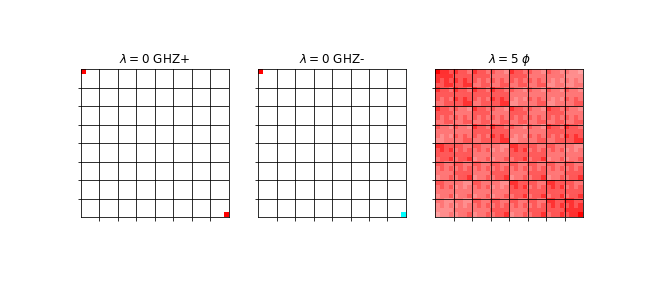
\includegraphics[width=\linewidth]{degenerategrounds}
	\caption{Qubism Plot of the ground states of a TFIM with N=10 sites , the complex coefficients are represented by colors, the grid is obtained iteratively. The states are the predicted ones.}
	\label{fig:lambdas}
\end{figure}\\
As expected in eq. \ref{eq:Ghz} and \ref{eq:phi}  for $\lambda=0$ the ground state is one of the $\ket{GHZ}$ states  and for $\lambda>>1$ the ground state is the product state $\ket{\phi}$ \\
The ground states show no dependence on the size of the model. \\
The ground states are not influenced by the boundary conditions (Open or Periodic) as long as the Hamiltonian is implemented in a symmetric fashion:
\begin{equation}
	H_{sym}=-\sum_{l}\left(\sigma_{l}^{z} \sigma_{l+1}^{z}+\frac{\lambda}{2}\sigma_{l}^{x}\sigma_{l+1}^{0}+\frac{\lambda}{2}\sigma_{l}^{0}\sigma_{l+1}^{x}\right)	
\end{equation}\\
With this prescription, every site is influenced by the external field. Even if the boundary sites feel only half his value the ground state doesn't change in an appreciable way.\\
If we are not careful, for small values of lambda the algorithm fails to preserve the $Z2$ symmetry. (fig.\ref{fig:randomdiag} )\\ 
As we said in eq. \ref{eq:lambda0}, for $\lambda=0$ every combination of the two ordered states is a possible groundstate. The Lanczos Algorithm \cite{Lanczos:1950} starts from a random vector $v_0$ and only needs to access the function:
\begin{equation}
	\ket{v_0} \mapsto H \ket{v_0}
\end{equation}
without having to write the full (huge) Hamiltonian.
Then with a kind of "steepest-descent" method, it finds a minimum. Nothing prevents the algorithm to break the symmetry. One solution is to force the algorithm to start from a symmetric vector (fig \ref{fig:correctdiag} )

\begin{figure}[h!]
	\begin{subfigure}{0.5\textwidth}	
	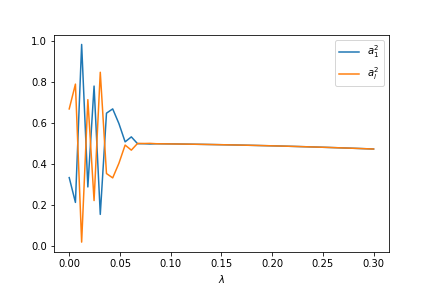
\includegraphics[width=\linewidth]{randomdiag}
	\caption{Random starting vector}
	\label{fig:randomdiag}
	\end{subfigure}
	\begin{subfigure}{0.5\textwidth}
	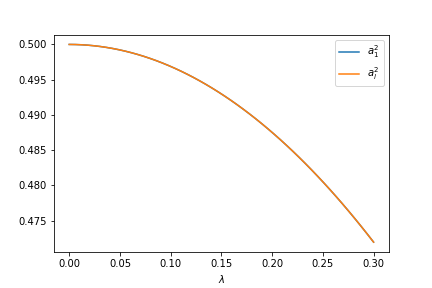
\includegraphics[width=\linewidth]{correctdiag}
	\caption{Symmetric starting vector}
	\label{fig:correctdiag}
	\end{subfigure}
\caption{First and last coefficients in the z-basis squared of the ground state. N=10 sites,  TFIM.}
\end{figure}


\subsection{DMRG Diagonalization}
With the DMRG algorithm \cite{De_Chiara_2008} keeping track of the groundstate wave-function it's not easy. One thing we can easily have access to is the density matrix $\rho_2$ of the two sites in the middle of the chain.\\
If the ground state is one of the $\ket{GHZ}$ states, then:
\begin{equation}
	\rho_2=\Tr_{N-2}(\ket{GHZ}\bra{GHZ})=\frac{1}{{2}}(\ket{\uparrow\uparrow}\bra{\uparrow\uparrow}+\ket{\downarrow\downarrow}\bra{\downarrow\downarrow})=\left[\begin{array}{cc}
		1/2 &  \\
		& 1/2
	\end{array}\right]	
\end{equation}
If instead the entanglement is lost:
\begin{equation}
	\rho_2=\left[\begin{array}{cc}
		1 &  \\
		& 0
	\end{array}\right]	 \text{or} \left[\begin{array}{cc}
	0 &  \\
	& 1
\end{array}\right]
\end{equation}
So to check if the ground state is one of the $\ket{GHZ}$ state we  can plot the "corner  coefficients" ($\rho_2^{00}$ and $\rho_2^{11}$) \footnote{We could also  plot the Entropy}.\\ We plot the "corner coefficients" against the size for different values of $\lambda$  \ref{fig:lambdaandsizes}. 
An interesting phenomenon happens: when we reach a certain size $N_{break}$ of the chain, the entanglement vanish. $N_{break}$ grows with $\lambda$.\\
I think that to explain this we have to consider that for small $\lambda$  we can treat the transverse term $V$ of the Hamiltonian as a perturbation:
\begin{equation}\label{eq:perturb}
	H_{QI}=H_0+V=-\sum_{l}\left(\sigma_{l}^{z} \sigma_{l+1}^{z}\right) - \lambda \sum_l  \sigma_{l}^{x}
\end{equation}
if we consider the amplitude at the k-th order in the perturbation:
\begin{equation}
	p=\bra{\uparrow...\uparrow}V^k\ket{\downarrow...\downarrow}=\begin{cases}
		0 \quad \text{if} \quad k<N\\
		\lambda^N \quad \text{if} \quad k=N
	\end{cases}
\end{equation}
We realize that when p it's too small, if we end up in one of the two completely ordered state we will never return to a $\ket{GHZ}$ state.\\
This will happen for some $N_{break}>\log\lambda_0  / \log \lambda $ with $\lambda_0$ some very small number.\\ If we instead are in a $\ket{GHZ}$ state there is always a non-zero probability of ending up in an ordered state.\\
This also proves that for $0<\lambda<1$ and large enough N, the ground state is one of the completely ordered states.
\begin{figure}[h]
	\hspace*{-4cm}
	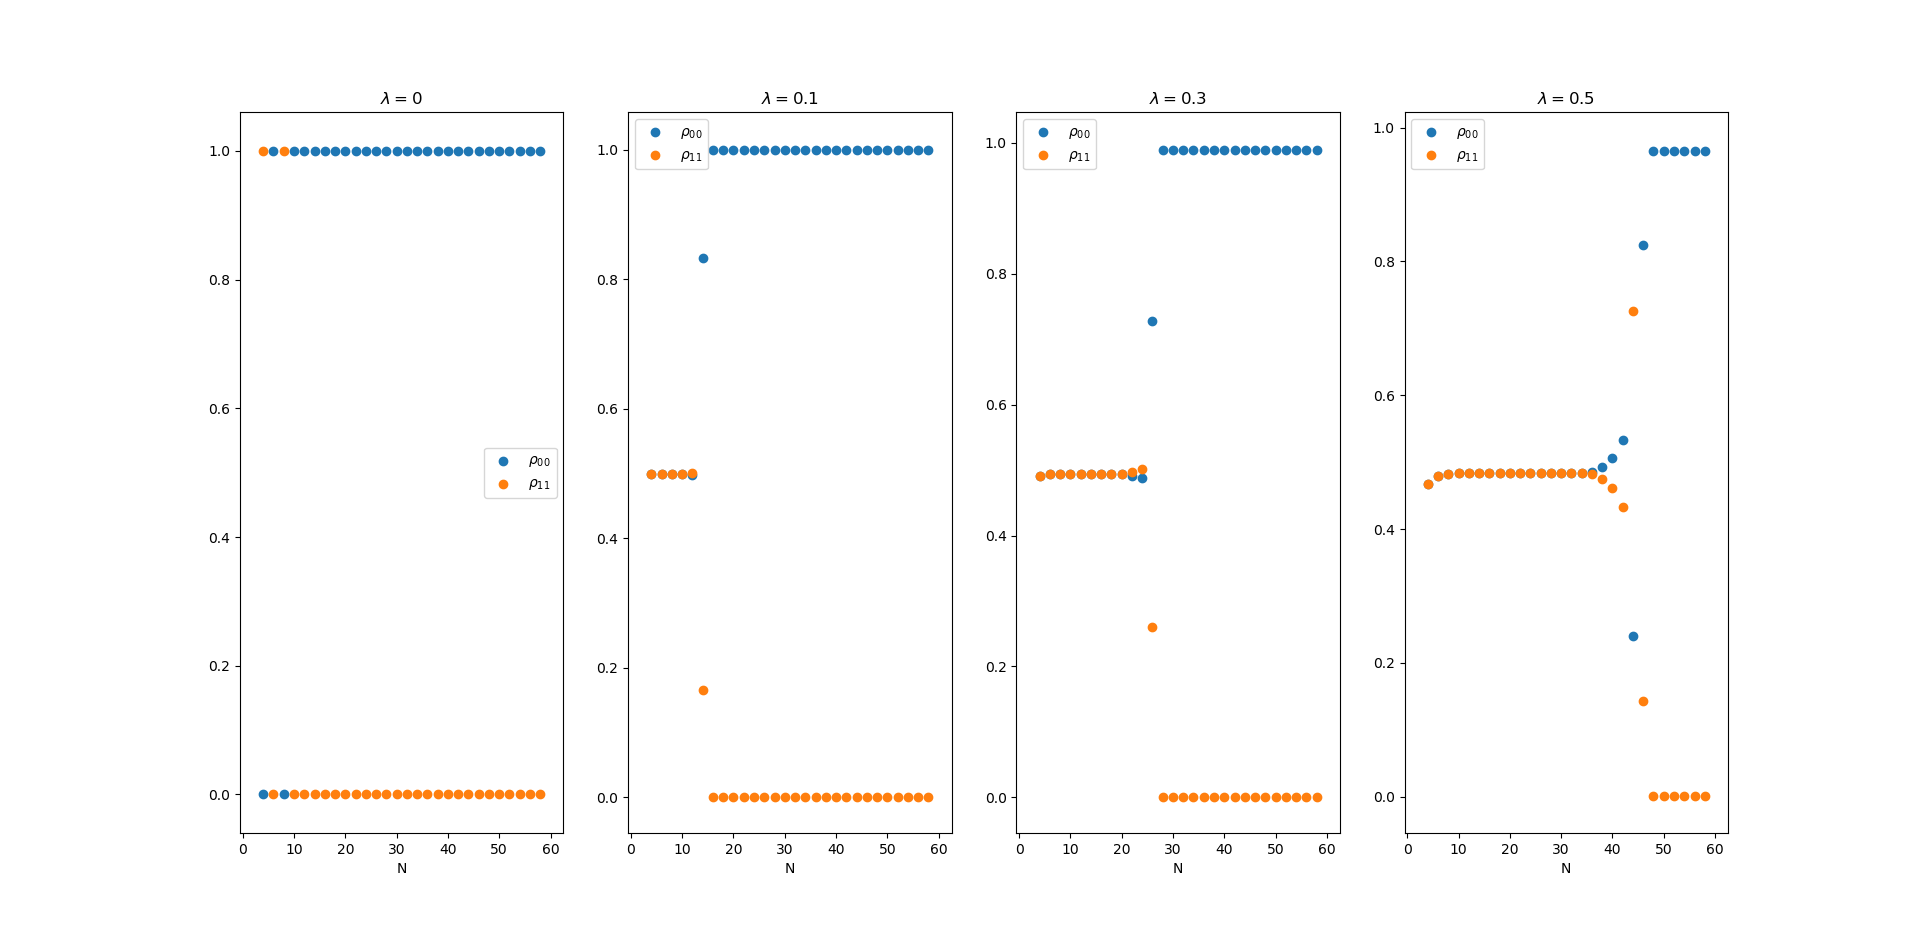
\includegraphics[width=1.5\linewidth]{lambdaandsizes}
	\caption{$\rho_2$ corners coefficients dependence on size for different values of $\lambda$ (iDMRG, m=20) }
	\label{fig:lambdaandsizes}
\end{figure}
\section{The Quantum-to-Classical mapping}
\newpage
\appendix
\section{Spontaneous symmetry breaking in the 2D Ising Model}
To study the temperature dependence of the 2D Ising model \ref{eq:hamiltclass} we assign to every configuration $\sigma$ of the variables the Boltzmann Distribution:
\begin{equation}
	P_{\beta}(\sigma)=\frac{e^{-\beta H(\sigma)}}{Z_{\beta}}
\end{equation} 
Simulating the model is a classic application of the Monte Carlo Method it is found that at low temperatures, even if $h=0$, the system becomes "magnetized": meaning that all the variables take the same value $+1$ or $-1$.\\ We also notice that if the size of the lattice is small the simulation alternates between the two values. For large sizes, the system gets stuck in one of the two ordered states. \\
This is an example of Spontaneous Symmetry Breaking (SSB): the $h=0$ Hamiltonian is clearly  symmetric under sign inversion: symmetry and translational invariance imply $\langle s \rangle=0$, yet at low temperature (and large enough size) $\langle s \rangle \ne 0$.  \\ 
How can we explain this behavior?\\
The model \ref{eq:hamiltclass} has been exactly solved by Onsager \cite{Huang_1987} and the magnetization has been calculated by Yang \cite{PhysRev.85.808}. These solutions are quite complicated but in this context we can say that the symmetry breaking stems from the following argument:\\
The limit function of a sequences of analytic function need not to be analytic, so the thermodynamic limit of the partition function can show some non-analytic behavior. \\ 


\subsection{Mean field Approximation}\label{MFA}
The MFA for the Ising Model it's also called Bragg-Williams Approximation, it's a crude way to simplify the Ising Hamiltonian but it's qualitatively correct in 2D
\begin{equation}
	s_i =  \left\langle s_{i}\right\rangle +\delta s_i 
\end{equation} 
We neglect the quadratic corrections in $\delta s$:
\begin{equation}
	s_{i} s_{j} \simeq \left\langle s_{i}\right\rangle\left\langle s_{j}\right\rangle+\left\langle s_{j}\right\rangle \delta s_{i}+\left\langle s_{i}\right\rangle \delta s_{j}
\end{equation}
The expectation value $\left\langle s_{i}\right\rangle=m$ for every site because the system is translationally invariant.\\
Consider the Hamiltonian \ref{eq:hamiltclass} with $h=0$:
\begin{equation}
	H_{CI}=-J\sum _{\langle i~j\rangle }s _{i}s _{j}
\end{equation}
If we apply the Mean Field Approximation:
\begin{equation}
	\mathcal{H}_{MF}=-J m \sum_{\langle i j\rangle}\left(s_{i}+s_{j}-m\right)
\end{equation}
In the 2D square-lattice every site has 4 nearest-neighbors, we sum to all the $N$ sites and  divide by two to avoid double-counting:
\begin{equation}
	\mathcal{H}_{MF}=-2 J m \sum_{i=1}^{N}\left(2 s_{i}-m\right) =2N J m^{2}-4 J m \sum_{i=1}^{N} s_i
\end{equation}  
With this Hamiltonian it's quite easy to calculate the partition function:
\begin{equation}
	Z_{MF} =\operatorname{Tr}\left(e^{-\beta \mathcal{H}_{MF}}\right) 
	=\prod_{i=1}^{N}\left(\sum_{s_{i}=\pm 1}\right) e^{-\beta \mathcal{H}_{MF}}=e^{-2 \beta N  J m^{2}}\left[2 \cosh \left(4 \beta Jm\right)\right]^{N}
\end{equation}
And from there the Free Energy:
\begin{equation}
	F_{MF}=-k_B T\ln Z_{MF}=2 N  J m^{2}-N k_B T\ln 2-N k_B T \ln \left[ \cosh \beta  4Jm \right]
\end{equation}
Expanding in powers of the mean-magnetization $m$ and defining $k_{\mathrm{B}} T_{c} \equiv 4 J$ we obtain:
\begin{equation}
	f(m)=\frac{F_{MF}}{N} \simeq F_{0}+\frac{k_BT_c}{2T}\left(T-T_{c}\right) m^{2}+\frac{k_BT_c^4}{12T^3} m^{4}= F_{0}+a(T)\left(T-T_{c}\right) m^{2}+b(T) m^{4}
\end{equation}
From simple calculations we can also write a condition on the mean-magnetization:
\begin{equation}
	m=\tanh [\beta(4J m)]
\end{equation}
$\beta \rightarrow +\infty$ $\implies$ $m\rightarrow \pm 1$

\subsection{Landau Theory}
We can get a intuitive (but only qualitative) idea of what's happening using the Landau Theory of Symmetry Breaking.  
It can be shown (\ref{MFA} ) that under some approximation the free energy density of the 2D Ising Model can be expressed as:
\begin{equation}
	f(m) \simeq f_{0}+a(T)\left(T-T_{c}\right) m^{2}+b(T) m^{4}
\end{equation}
Where:
\begin{equation}
	m=\langle s_i \rangle = \frac{\sum_{\sigma} s_i e^{-\beta H(\sigma)}}{Z_{\beta}}
\end{equation}
Is the mean magnetization at temperature $T=1/k_B\beta$.\\
This Free Energy give rise to the familiar "Mexican Hat" of the Landau Theory of symmetry breaking.( fig. \ref{fig:landau} )\\
\begin{figure}[h!]
	\centering
	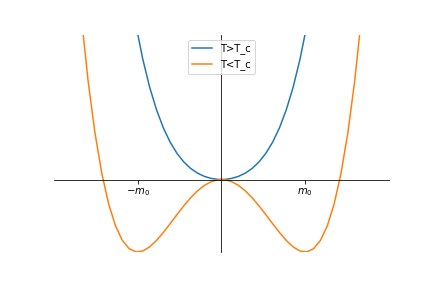
\includegraphics[width=0.7\linewidth]{landau}
	\caption{$f-f_0$ for different Temperatures}
	\label{fig:landau}
\end{figure}\\
Looking at the figure we conclude that:
\begin{enumerate}
	\item When $T<T_c$ two new ground states appear with a non-zero magnetization
	\item The new ground states have opposite values of m
\end{enumerate}
We now have an easy explanation of the SSB: when $T<T_C$ the state with zero total magnetization becomes unstable and the sistem goes to one of the two magnetized ground state. \\ For $T \rightarrow 0$ the mean magnetization of the degenerate ground states: $m_0\rightarrow \pm1$ (\ref{MFA}).
This last point explains why at large sizes the system gets stuck: even if the transition between the states costs no energy, it requires the system to flip simultaneously all the variables, an event that becomes extremely unlikely at large sizes.
\section{Simmetry Breaking in the Quantum Ising model (notes to improve)}
We'll do time-independent perturbation theory for an Hamiltonian with a degenerate groundstate:
\begin{equation}
	|\psi\rangle=\sum_{\alpha} c_{\alpha}|\alpha\rangle+\sum_{k} d_{k}|k\rangle
\end{equation}
Psi is the perturbed eigenstate Greek letters on the degenerate space, roman letters outside.\\
We suppose that $d_k$ are at least at the first order in $\lambda$
\begin{equation}
	\sum_{\alpha}\left(H_{0}-E+V\right) c_{\alpha}|\alpha\rangle+\sum_{k}\left(H_{0}-E+V\right) d_{k}|k\rangle=0
\end{equation}
Multiply on the left by $\bra{\beta}$ and $\bra{j}$:
\begin{equation}\label{eq:degen}
		\sum_{\alpha}\left\langle\beta\left|\left(H_{0}-E+V\right)\right| \alpha\right\rangle c_{\alpha}+0+ \\
		\sum_{k}\langle\beta|V| k\rangle d_{k}=0
\end{equation}
\begin{equation}\label{eq:ortho}
		0+\sum_{\alpha}\langle j|V| \alpha\rangle c_{\alpha}+\left(E_{j}-E\right) d_{j}+ \\
		\sum_{k}\langle j|V| k\rangle d_{k}=0
\end{equation}
Neglect second order correction:
\begin{equation}\label{eq:secular}
	\left(\left(E_{0}-E\right) \delta_{\alpha \beta}+V_{\beta \alpha}\right) c_{\alpha}=0
\end{equation}
If we manage to solve this equation  \ref{eq:secular} and find the corrected Energy E, we can put it in \ref{eq:ortho} to find the coefficients on the orthogonal space:
\begin{equation}\label{eq:correction}
	d_{j}=\frac{1}{E-E_{j}} \sum_{\alpha}\langle j|V| \alpha\rangle c_{\alpha}
\end{equation}
If we now put this $d_j$ in eq. \ref{eq:degen} this is the second order:
\begin{equation}
	\sum_{\alpha}\left\langle\beta\left|\left(E_{0}-E+V\right)\right| \alpha\right\rangle c_{\alpha}+\sum_{k} \frac{\langle\beta|V| k\rangle\langle k|V| \alpha\rangle}{E-E_{k}} c_{\alpha}=0
\end{equation}
In our case \ref{eq:perturb}:
\begin{equation}
	H_{QI}=H_0+V=-\sum_{l}\left(\sigma_{l}^{z} \sigma_{l+1}^{z}\right) - \lambda \sum_l  \sigma_{l}^{x}
\end{equation}
if $\alpha=\ket{up}$ then 
\begin{equation}
	V\ket{\alpha}=\lambda\sum_{ l }( \ket{\downarrow}_l\ket{up_{N-1}})
\end{equation}
So if $\beta=\ket{down}$ we have :
\begin{equation}
	\bra{\beta}V=\lambda\sum_{ l }( \bra{\uparrow}_l\bra{down_{N-1}})
\end{equation}
so if we write:
\begin{equation}
\Delta_E=\sum_{k} \frac{\langle\beta|V| k\rangle\langle k|V| \alpha\rangle}{E-E_{k}} c_{\alpha}=0
\end{equation}
because projector on different states\\
What happens if we choose:
$\gamma=(1/\sqrt(2)(\ket{up}+\ket{down})$ ,$\delta=(1/\sqrt(2)(\ket{up}-\ket{down})$?
\begin{equation}
	\Delta_E=\sum_{k} \frac{\langle\beta|V| k\rangle \langle k |V| \beta \rangle+\langle\beta|V| k\rangle\langle k|V| \alpha \rangle-\langle\alpha|V| k\rangle\langle k|V| \beta\rangle+\langle\alpha|V| k\rangle\langle k|V| \alpha\rangle}{E-E_{k}} c_{\alpha}
\end{equation}
\begin{equation}
	\Delta_E=\sum_{k} \frac{\langle\beta|V| k\rangle \langle k |V| \beta \rangle+\langle \alpha |V| k\rangle\langle k|V| \alpha\rangle}{E-E_{k}} c_{\alpha}=\sum_{k} \frac{\lambda^2}{E-E_{k}} c_{\alpha}= \frac{N\lambda^2}{E-E_{k}} c_{\alpha}
\end{equation}
So GHZ states have a correction at the second order, the ordered states don't have perturbative corrections up to the $N$-th order
\bibliographystyle{alpha}
\bibliography{bibdeg}

\end{document}